\begin{figure}[h]
   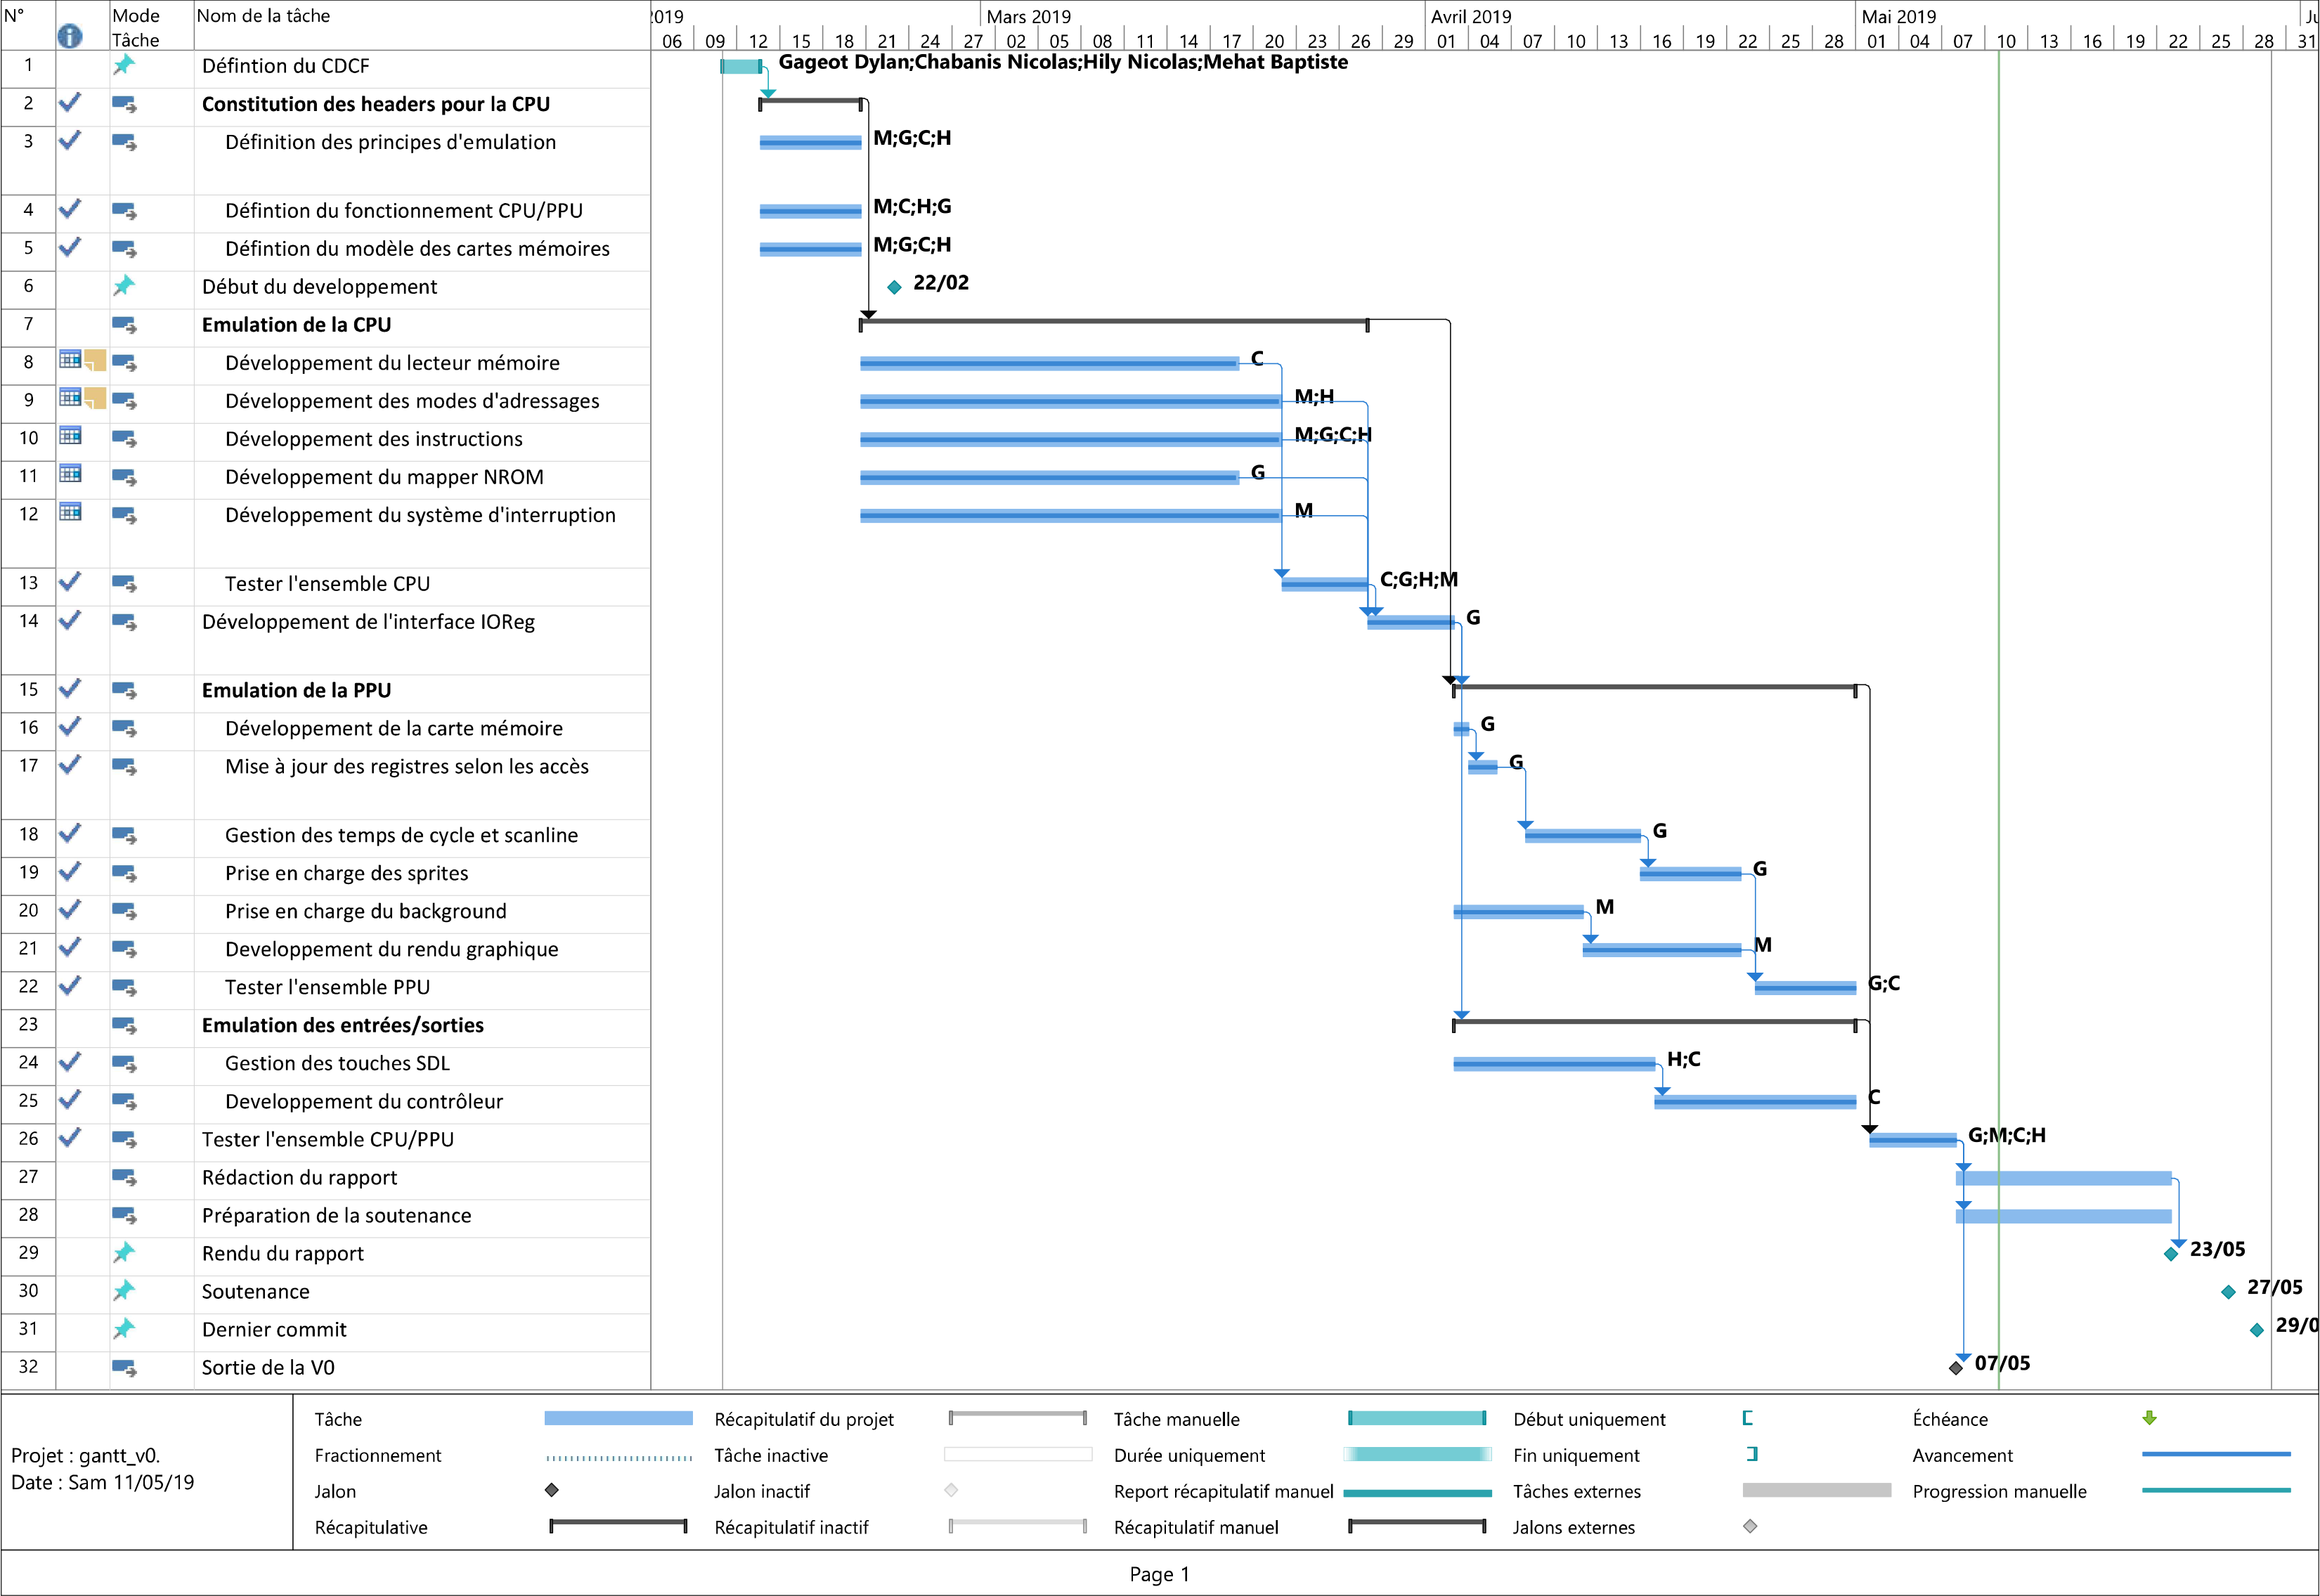
\includegraphics[scale=0.45]{GantV2.png}
   \caption{\label{étiquette} Diagramme de Gant de fin de Projet}
\end{figure}

\emph{  Comme vous pouvez le voir en comparant le diagramme de gant du début de projet et celui de fin de projet, celui ci s'est deroulé en deux étapes contrairement au trois prévues. Le devellopemet de la CPU a été fait dans les échéances souhaités. Cependant, par la suite, il a été décidé de revoir l'organisation sur le devellopemet de la PPU et de l'IHM. En effet, lors de l'étude de la PPU, il est apparu plus simple que seulement deux personnes s'en occupent du fait de la compléxité des liens existants entre chaques fonctions codées. Ainsi la PPU a été confié à Dylan et Baptiste alors que Nicolas C et Nicolas H se sont concentrés sur la gestion de touches avec la SDL et le controleur. C'est donc le 7/05 que la V0 a été crée contrairement 29/04. La V1 contenant l'IHM a été totalement mis à l'écart de fait de la trop grande quantité de temps que cela demandait.}
